\documentclass[titlepage]{article}
\usepackage{graphicx}
\title{Final Assignment:\\Integration of Tools and Practices}
\author{Mohammad Yavari}
\begin{document}
\maketitle
\tableofcontents
\pagebreak
\section{Git and GitHub:}
\subsection{Repository Initialization and Commits}
on GitHub, New Repository, Give it a Name, Clone it into Your PC (e.g. using the https link and git clone command), Create a main.tex file and .github/workflows/main.yml (further explained).
\subsection{ GitHub Actions for LaTeX Compilation}
first I did'nt know about the tags so I tried to do it on every push and remove the tag condition but when I discovered the releases that are created automatically and went through some difficulties and problems
I/ learned tags and I'm happy about it!\newline
you simply need to use the command git tag after the commit you want to be complied and then push using git push origin tagname\newline
(I did'nt changed the main.yml file) 
\section{Exploration Tasks}
\subsection{Vim Advanced Features}
\begin{enumerate}
\item Multiple Cursors with Visual Mode:\\
Vim allows you to use visual mode to create multiple cursors and edit multiple occurrences simultaneously.\\
Use Ctrl+v to enter visual block mode.\\
Move to select the desired columns or lines.\\
Press I to insert text simultaneously on all selected lines.\\
Press Esc to apply changes.
\item Folding:\\
Vim supports code folding, allowing you to collapse and expand sections of your code. This is beneficial for navigating large files or focusing on specific parts of the code.\\
zf followed by a motion: Create a fold.\\
zo and zc: Open and close folds, respectively.\\
:set foldmethod=indent: Automatically fold based on the indentation.\\
\item Marks and Jumps:\\
Marks allow you to bookmark a location in a file. You can set a mark with m{letter}, and then jump to that mark with `{letter}.\\
ma: Set mark a at the current cursor position.\\
`a: Jump to the position of mark a.\\
Jumps can be used to quickly navigate between different parts of your file. Vim also has a "jump list" (:jumps) that keeps track of recent cursor movements.
\end{enumerate}
\subsection{Memory profiling}
Normally C stores data in static mode (as I know), it has pros and cons, it's more stable and reliable and also easier but gives us less control, if we want control and flexibility we can use dynamic memory allocation
which we can use by functions like malloc / calloc / realloc / free, \newline the syntax and usage are so simple!
\subsubsection{Memory Leak}
a memory leak happens when your program forgets to return the borrowed space. It's like borrowing a pen but never giving it back. If you keep doing this, you run out of pens, and your backpack gets heavy with stuff you don't need.\newline
in other words, remember to free() after allocation!
\subsubsection{Memory profilers}
\paragraph{Memory Leak Detection:}
Valgrind keeps track of every allocation and deallocation of memory during the execution of a program.\\
If your program forgets to free up memory (a memory leak), Valgrind will point it out. It tells you where the leak occurred and how much memory is involved.
\paragraph{Memory Corruption Detection:}
Valgrind can detect issues like accessing memory beyond its boundaries, which can lead to unpredictable behavior and crashes.(Like in arrays in c)\\
If your program writes to or reads from memory it shouldn't, Valgrind can catch these errors.
And More...
\subsection{GNU/Linux Bash Scripting}
\subsubsection{fzf}
Fuzzy searching is like having a helpful friend who finds what you're looking for even if you don't know the exact details. It's a search technique that doesn't demand precision. Instead, it accommodates small mistakes, typos, or variations in spelling.
\\ it brings "fuzziness into the search"!
\\\\
it takes the list of files and directories from the ls command and allows you to interactively search and select one of them using a fuzzy search algorithm.\\
when you start typing it starts searching and highlighting a result!
\subsubsection{Using fzf to find your favorite PDF}
1. fd -e pdf\\
2. fd -e pdf | fzf
\subsubsection{Opening the file using Zathura}
zathura "\$(fd -e pdf | fzf)"
\section{Git and FOSS}
\subsection{Issues}
\begin{figure}[h]
	\centering
	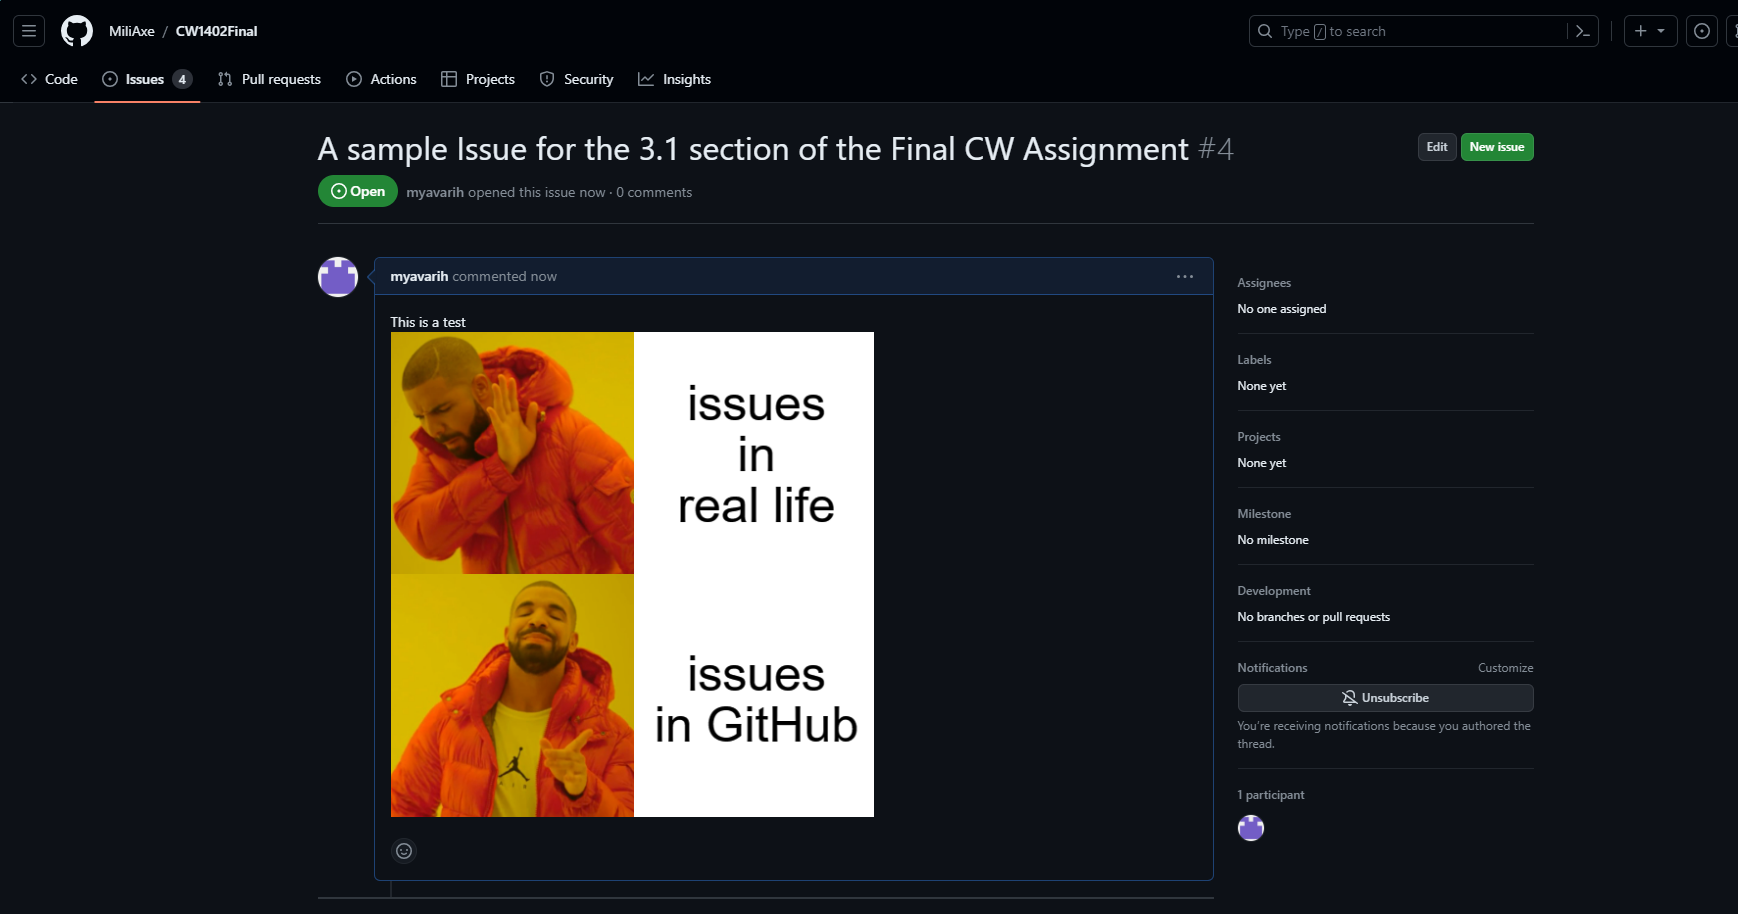
\includegraphics[width=0.7\linewidth]{screenshot001}
	\caption{Sample Issue}
	\label{fig:screenshot001}
\end{figure}

\end{document}